\documentclass[10pt,conference,letterpaper]{IEEEtran}


%\usepackage[latin1]{inputenc}   % for Latin languages
%\usepackage[T1]{fontenc}    % for ISO and UTF characters
%\usepackage[english]{babel} % for multilingual support

\usepackage{times}
\usepackage{color}
\definecolor{Red}{rgb}{.9,0,0}

\usepackage{amsmath,epsfig}
\usepackage{listings}
%\usepackage{verbatim}
\usepackage{alltt}
\usepackage{fancyvrb}
\usepackage{xspace}
\usepackage{multirow}
\usepackage{booktabs}
\usepackage{subfig}

\usepackage{todonotes}
% correct bad hyphenation here
\hyphenation{op-tical net-works semi-conduc-tor}

\usepackage{listings}
\lstset{keywordstyle=\bfseries, flexiblecolumns=true}
\lstloadlanguages{C,[ANSI]C++,HTML}

%------------------------------------------------------------------------- 
% take the % away on next line to produce the final camera-ready version 
%\pagestyle{empty}

%------------------------------------------------------------------------- 
\newtheorem{lemma}{Lemma}
\newtheorem{theorem}{Theorem}
\newtheorem{definition}{Definition}
\newtheorem{heuristic}{Heuristic}
\newtheorem{prop}{Proposition}

% Commands
\newcommand{\tuple}[1]{\langle #1 \rangle}
\newcommand{\hdp}[1]{{\color{red}\textbf{HDP:}#1}}
\newcommand{\ara}[1]{{\color{blue}\textbf{ARA:}#1}}

\newcommand{\iadd}{{\sf\small add}\xspace}
\newcommand{\sleq}{{\sf\small subleq}\xspace}
\newcommand{\sleqs}{{\sf\small subleq }}
\newcommand{\sleqi}{{\sf\small subleqi}}
\newcommand{\sleqis}{{\sf\small subleqi }}
\newcommand{\ur}{{URISC}}
\newcommand{\urs}{{URISC }}
\newcommand{\urisc}{{\sf\small MIPS-URISC}}
\newcommand{\uriscs}{{\sf\small MIPS-URISC }}
\newcommand{\tiger}{{TigerMIPS}}
\newcommand{\tigers}{{TigerMIPS }}
\newcommand{\exwb}{{\sf\small ExWb}}
\newcommand{\exwbs}{{\sf\small ExWb }}
\newcommand{\fstage}{{\bf\small Fetch}}
\newcommand{\dstage}{{\bf\small Decode}}
\newcommand{\estage}{{\bf\small Execute}}
\newcommand{\mastage}{{\bf\small Memory Access}}
\newcommand{\wbstage}{{\bf\small Writeback}}
\newcommand{\exwbstage}{{\bf\small ExecuteWriteback}}
\newcommand{\fstages}{{\bf\small Fetch }} 
\newcommand{\dstages}{{\bf\small Decode }}
\newcommand{\estages}{{\bf\small Execute }}
\newcommand{\mastages}{{\bf\small Memory Access }}
\newcommand{\wbstages}{{\bf\small Writeback }}
\newcommand{\exwbstages}{{\bf\small ExecuteWriteback }}
\newcommand{\scom}{{subtract and compare}}
\newcommand{\scoms}{{subtract and compare }}
\newcommand{\urwritereg}{{\sf\small writeRegDataWB}}
\newcommand{\urwriteregs}{{\sf\small writeRegDataWB }}
\newcommand{\urlteqz}{{\sf\small lteqz}}
\newcommand{\urlteqzs}{{\sf\small lteqz }}
\newcommand{\mfu}{{\sf\small mfu}}
\newcommand{\mfus}{{\sf\small mfu }}
\newcommand{\mtu}{{\sf\small mtu}}
\newcommand{\mtus}{{\sf\small mtu }}


\newcommand{\fig}[4][htbp]{
  \begin{figure}[#1] {\centering\scalebox{#2}{\includegraphics{fig/#3}}\par}
    \caption{#4\label{#3}}
  \end{figure}
}

\newcommand{\multfigtwoh}[6][htbp]{
\begin{figure*}[#1]
  \centering
  \subfloat[]{\label{#3}\scalebox{#2}{\includegraphics{fig/#3}}}
  \subfloat[]{\label{#4}\scalebox{#2}{\includegraphics{fig/#4}}}
  \caption{#6}
  \label{#5}
\end{figure*}
}

\newcommand{\multfigtwov}[6][htbp]{
\begin{figure}[#1]
  \centering
  \subfloat[]{\label{#3}\scalebox{#2}{\includegraphics{fig/#3}}}\\
  \subfloat[]{\label{#4}\scalebox{#2}{\includegraphics{fig/#4}}}
  \caption{#6}
  \label{#5}
\end{figure}
}

\newcommand{\figR}[5][htbp]{
  \begin{figure}[#1]{\centering\scalebox{#2}{\includegraphics[angle=#5]{fig/#3}}\par}
    \caption{#4\label{#3}}
  \end{figure}
}

\newcommand{\figTC}[4][htbp]{
  \begin{figure*}[#1] {\centering\scalebox{#2}{\includegraphics{fig/#3}}\par}
    \caption{#4\label{#3}}
  \end{figure*}
}

\newcommand{\figEMPTY}[5][htbp]{
  \begin{figure}[#1]
    \fbox{\begin{minipage}{#2}\hfill\vspace{#3}\end{minipage}}
    \centering
     \label{#4}
    \caption{#5}
  \end{figure}
}

\newcommand{\tab}[3][htbp]{
  \begin{table}[#1]
    \footnotesize
    \centering
    \caption{#3}
    \include{tab/#2}
    \label{#2}
  \end{table}
}

\newcommand{\tabTC}[3][htbp]{
  \begin{table*}[#1]
    \footnotesize
    \centering
    \caption{#3}
    \include{tab/#2}
    \label{#2}
  \end{table*}
}



\newcommand{\head}[1]{\textnormal{textbf{#1}}}



\setlength{\intextsep}{8pt}
\setlength{\floatsep}{8pt}
\setlength{\dblfloatsep}{8pt}
\setlength{\abovecaptionskip}{3pt}
\setlength{\belowcaptionskip}{1pt}

\begin{document}

\title{RTSNoC: A Predictable Network-on-Chip for Real-time Applications}

\author{
\begin{tabular}{cc}
Marcelo D. Berejuck , Ant{\^{o}}nio A. Fr{\"{o}}hlich, Tiago R. M{\"{u}}ck & Hiren D. Patel\\
Federal University of Santa Catarina & University of Waterloo\\
Florian\'{o}polis, Brazil & Waterloo, Canada\\
\{berejuck,guto,tiago\}@lisha.ufsc.br & hdpatel@uwaterloo.ca
\end{tabular}
}

\maketitle

\begin{abstract}
We present the design and analysis of a predictable network-on-chip (NoC) interconnect for real-time applications, which we call RTSNoC. RTSNoC is specifically designed to allow predicting the worst-case latencies of any data flowing through the interconnect. It uses wormhole switching with alterations such that  every flit carries  routing information. The routers use this information to perform runtime arbitration and schedule the flits to the corresponding output ports while preventing contention on the communication channel. We implement RTSNoC on an FPGA, and utilize it in building a prototype SoC with multiple processors communicating across RTSNoC. We compare with another prototype SoC using the same multiple processor communicating approach, however, across a Time-Division Multiplexing (TDM) NoC. Our implementation shows that RTSNoC has better performance than TDM approach at high traffic flow, and it is a cost-effective solution to scalability of the system.
\end{abstract}

\begin{keywords}
Network-on-Chip, Real-time system, Field-programmable gate array.
\end{keywords}

\begin{figure*}[htbp]
\centering
\subfloat[RTSNoC router. Each corner is a point of connection to the network.]{
	\label{RTSNoC_Figure_1}
	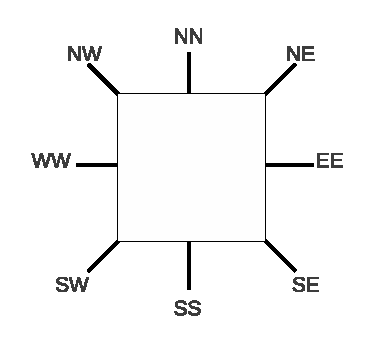
\includegraphics[width=.35\columnwidth]{Figures/RTSNoC_Figure_1}
}
\quad
\subfloat[Communication channel signals.]{
	\label{RTSNoC_Figure_2}
	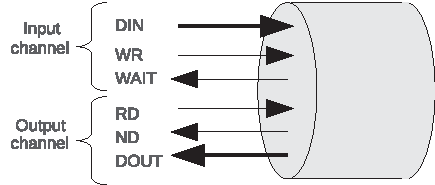
\includegraphics[width=.55\columnwidth]{Figures/RTSNoC_Figure_2}
}
\quad
\subfloat[A regular mesh NoC with 4 routers and 24 cores.]{
	\label{RTSNoC_Figure_4}
	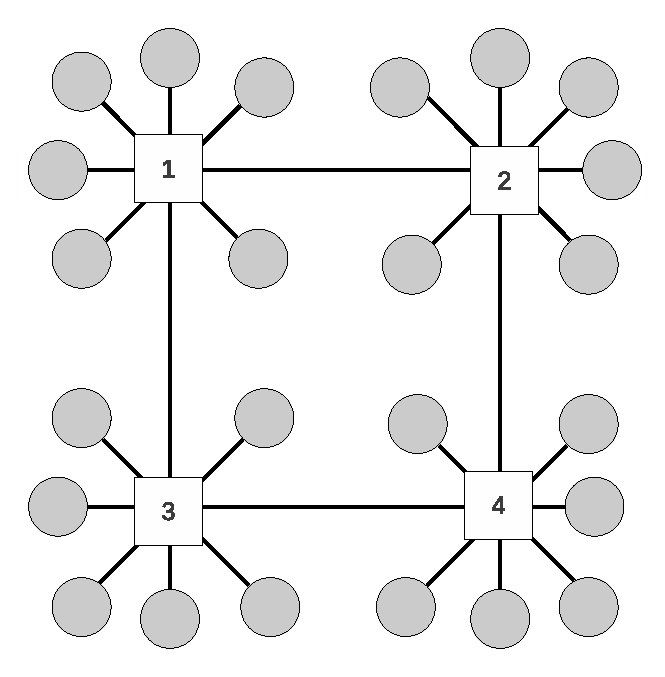
\includegraphics[width=.35\columnwidth]{Figures/RTSNoC_Figure_4}
}
\caption{RTSNoC components.}
\label{fig:rtsnoc}
\end{figure*}


\section{Introduction}
\label{sec:introduction}

Deploying real-time applications on modern SoCs mandates that the designer ensures performance and temporal guarantees. While performance guarantees are provided through testing, temporal guarantees require predicting the worst-case execution times (WCETs) of the application when executing on the SoC.
Note that modern SoC platforms typically consist of multiple processors, and a communication interconnect between them. A popular communication interconnect is a network-on-chip (NoC), which provides a scalable, reusable, and an efficient interconnect. However, predicting WCETs of applications on such SoCs becomes difficult when using off-the-shelf processors, and NoCs. This is because off-the-shelf solutions primarily focus on improving the average-case performance whereas real-time applications necessitate temporal guarantees to ensure correctness. As a result, there has been considerable interest in the design of predictable real-time processors~\cite{lickly:08:cases}, and predictable real-time NoCs~\cite{Goossens:2005:NCC:1092232.1092305,Shi:2008}. In this work, we restrict our focus to the communication interconnect, and in particular we propose the design of a predictable NoC for real-time applications called RTSNoC.

There are two broad categories of real-time NoCs: resource reservation and runtime arbitration.
The principle behind resource reservation techniques is to pre-allocate resources and schedule the communication using these resources so as to guarantee that temporal requirements are met.  
One such example uses time-division multiplexing (TDM)~\cite{Goossens:2005:NCC:1092232.1092305, Zeferino:2003:SPS:942808.943980}. TDM NoCs require an allocation algorithm to statically schedule packet transmissions each cycle from the source to the destination by generating a slot table for each router. 
This has the advantage that determining the WCET for communication is simple. The disadvantage, however, is that TDM requires pre-allocation of resources, and a slot allocation algorithm. 
To counter the issue of pre-allocation of resources, an alternative proposal uses runtime arbitration~\cite{Shi:2008} where the routers are aware of priorities, and there are distinct virtual-channels (VCs) for each priority level.  Flits in the same router competing for the same output port enter arbitration where the one with the highest priority gets routed to the output. The advantage of runtime arbitration is that there is no need to schedule flit transmissions, but there is a need to statically analyze the WCETs. Furthermore, the requirement of a separate VC for each priority level will incur significant resource overheads.

In efforts to design a real-time NoC that is predictable yet one that is efficient in its implementation, we present a real-time service NoC (RTSNoC). RTSNoC uses a connectionless technique that is predictable; thereby, allowing designers to predict WCETS. The RTSNoC implements a regular 2-D mesh in which each router can connect up to eight processing cores. For the RTSNoC, we introduce extra routing information to each flit. The RTSNoC routers implement a priority-based dynamic round-robin algorithm, which use the extra information in the flits to govern its path through the NoC. This algorithm prevents channel contention, and keeps a uniform latency for all requests, while yielding a fixed maximum latency regardless of the network load. We implement RTSNoC on an FPGA, and compare it with a similar implementation using another network called SoCIN \cite{Zeferino:2003:SPS:942808.943980} that implements TDM. Both network were done with several cores generating random traffic to a same destination core. That traffic was increased by steps up to 100 \% of offered traffic, and the latency and jitter were evaluated for both cases.
%\todo[inline]{Add information about what you compare with, and what case study you design}

The remaining of this paper is organized as follows: Section \ref{sec:related_work} presents a discussion about network implementations that exploit connection-oriented techniques; Section \ref{sec:rtsnoc} presents RTSNoC architecture and its WCET analysis, along with a comparison between RTSNoC and a traditional TDM-based NoC; Section \ref{sec:evaluation} evaluates the impact of the proposed mechanisms in terms of silicon area, latency, and jitter; Section \ref{sec:case_study} presents the deployment of RTSNoC in a FPGA-based \textit{Private Automatic Branch eXchange}~(PABX) SoC; and Section \ref{sec:conclusion} closes the paper with our conclusions.


\section{Related Work}
\label{sec:related_work}

There exist NoCs designed to provide worst-case latency guarantees on the communication. Examples of such NoCs are AEthereal~\cite{Goossens:2005:NCC:1092232.1092305} and dAElite~\cite{dAElite}. AEthereal uses TDM techniques to create dedicated channels that provide contention-free routing, and it provides guaranteed worst-case latency bounds. With TDM, the bandwidth of each link is split into a predefined number of time slots at design-time. This is dependent on the communication traffic expected in the network. These time slots are then statically assigned to data transmissions such that entire flows of data can be transferred from its source to destination. Another NoC called TTNoC~\cite{TTNoC} offers more freedom than traditional TDM NoCs by supporting multicast and broadcast operations. Further, TTNoC provides tight worst-case latency guarantees; however, the network must be re-designed/configured to closely match the network load required by the application. Different applications may require a costly redesign of the network, which hinders the flexibility and scalability of the system. Nostrum~\cite{Millberg:2004:GBU:968879.969206} uses a different approach, and does not require a fixed TDM schedule. The TDM period is linked to the length of looping connections. Multicast is supported by adding more receiver nodes to a closed loop. Nostrum also offers BE communication using deflection routing. The disadvantage of Nostrum is that routing paths, and consequently multicast node sets must also be decided at design-time. The conceptual NoC in~\cite{Shi:2008} presents a priority-aware NoC where each flow entering a router has a unique priority, and thus, associated with a distinct virtual-channel. Routing is based on priorities when contentions for the same output port arise. We expect an implementation of this NoC to be expensive because the number of virtual-channels necessary changes with the application being deployed on the NoC. In addition, there does not exist a real implementation of this NoC.
%Other networks were originally designed as BE networks and latter extended with QoS mechanisms, like SoCIN~\cite{Zeferino:2003:SPS:942808.943980}. SoCIN incorporated a packet aging mechanism in which a packet receives an initial priority level when injected into the network. Increments in the priority level will occur according its permanence in the network~\cite{Berejuck:2009:AMQ:1601896.1601928}.

%Some networks provide explicit \textit{Quality-of-Service}~(QoS) mechanisms.
%QNoC~\cite{3:Bolotin:2003} splits flows into different categories, assigning different priorities
%for each one. Other networks, like SoCIN~\cite{Zeferino:2003:SPS:942808.943980} and
%Hermes~\cite{5:Moraes:2004}, were originally designed as BE networks and latter extended with QoS
%mechanisms. Hermes introduced a virtual channel mechanism, similar to the one proposed by
%\cite{Goossens:2005:NCC:1092232.1092305}. SoCIN incorporated a packet aging mechanism in which a
%packet receives an initial priority level when injected into the network. Increments in the priority
%level will occur according its permanence in the network~\cite{Berejuck:2009:AMQ:1601896.1601928}.

%On a different approach~\cite{6126723}, the authors claim that it is difficult to estimate
%the communication delay of NoC-based systems due to their complexity, making implementation of
%real-time systems on NoCs virtually impossible. They proposed a method for communication modeling
%and synthesis of dynamically reconfigurable NoC-based systems that enable contention-aware
%scheduling. The network model is defined at system-level, and the method to prevent against
%contention is an extension of the edge scheduling approach used in distributed
%systems~\cite{1425439}.

\section{The RTSNoC Architecture}
\label{sec:rtsnoc}
We describe the design of the wormhole-switched RTSNoC architecture, and how it lends itself to static WCET analysis to determine the worst-case communication latencies.

\subsection{Design}
The basic building block of an RTSNoC network is the router as shown in Figure~\ref{RTSNoC_Figure_1}. 
The RTSNoC router has eight interconnection points: north (NN), northeast (NE), east (EE), southeast (SE), south (SS), southwest (SW), west (WW), and northwest (NW). Each of these router interconnection points provides two unidirectional channels, and flow control signals as shown in \ref{RTSNoC_Figure_2}. We allow the size of each channel to be configurable based on the needs by the application. The signal bus called DIN and DOUT refer to input and output data bus, and the signals RD and WR are strobes used to read and write data. The signals WAIT and ND are used for flow control. WAIT informs that the processor must wait before writing new data to the router input channel, and the signal ND informs the destination that a new packet is available. Communication channels may be connected to processing cores or to other routers in order to build a 2D regular mesh network. Figure \ref{RTSNoC_Figure_4} illustrates an instance of a generic system implemented using the RTSNoC. Four routers are used to establish a $2 \times 2$ 2-D regular mesh network that can interconnect up to 24 cores. 

\figSC{.55}{RTSNoC_Figure_3}
{Block diagram showing the internal structure of the router}  

Figure \ref{RTSNoC_Figure_3} shows the internal router structure. 
Each communication channel has an input interface, an output interface, and a flow controller. 
The input interface has a register that stores a flit. 
When a processor transmits data through the network, it transforms the packets into flits and these flits are sent to the communication channel.
This register is where the flit gets stored when it is transmitted.
The flow controller assists in informing the arbiter of a new flit that needs to be routed. 
It also checks the flit header for its destination address, and verifies if the requested output channel in the router is ready to receive the flit. If the output channel is available, the flow controller sends a request to the arbiter using internal signals. Once the output signal receives the flit, it sets the ND signal and will be wait for a reading in the RD signal before to provide the flit in the connection link.

The \emph{arbiter} is an integral component of the router.  
It implements the runtime arbitration algorithm that ensures contention-free routing, which we describe with the help of Figure \ref{Arbiter}. 
During system startup, each channel receives a default unique priority level. 
The default priority assignment assigns priorities in descending order to the following channels: NN, SS, EE and WW. 
When a processor transmits a flit to its corresponding router's channel, if the channel has the highest priority then the arbiter forwards the flit to the requested output channel. 
This occurs whether there are no flits in the other channels or when there exist other flits waiting to be routed at other channels. 
Once the higher priority channel's request gets granted, and the flit forwarded, the algorithm reassigns the priorities to the channels.
The priority of the recently attended channel becomes the lowest priority, and for all other channels, the priority gets increased to the next highest priority level. 
This allows fairness in routing the flits in the router. 
Notice that when there is no contention for the output channel, a flit in a lower priority channel can be granted access to its output channel.
Hence, the arbitration is only necessary when there is contention for an output channel.
Upon granting a channel rights to forward its flit, the arbiter sends a command to the \emph{switch} block to actually perform the granted routing. 

\figSC{.45}{Arbiter}
{Flowchart showing the dynamic scheduling algorithm implemented in RTSNoC}  

In order to facilitate this runtime routing algorithm, RTSNoC uses a certain amount of control data that needs to be transmitted along with the data.
For RTSNoC, we require that each flit carries source and destination address in addition to the payload. 
Recall that traditional wormhole-switched NoCs have header flits that  contain the source/destination addresses for the packet. 
However, while the header flit travels through the network, it allocates virtual-channels through the network for the transmission of the remaining flits of the same packet until the tail flit frees up the virtual-channel. 
In our case, we allow the routing of each individual flit. 
We do this because, in this case, there is no need to allocate virtual-channels through the network, because all flit has routing information added to data and may be treated separately. Other NoCs usually sends a header flit with information routing and that flit will allocate the virtual-channels through the network. After that allocation, the packet body can be sent through the allocated path. O tail flit must be sent to inform all routers in the path that they may cancel the connections and let another flows to request them.

%\todo[inline]{Why do you want to route individual flits?}
We understand that there is a tradeoff when adding source/destination information to the flits, which is the increase in area due to wider data busses for each channel.
We show the packet format used in RTSNoC in Figure \ref{RTSNoC_Figure_5}.  
\figSC{.45}{RTSNoC_Figure_5}
{RTSNoC packet format. The size of X/Y fields depends on the topology.}  
Two fields called $X_{ORI}$ and $Y_{ORI}$  inform the X and Y coordinates of the network router where
the packet was generated (i.e. the origin address of the packet). The same happens to the destination
router that have the fields called $X_{DST}$ and $Y_{DST}$ to indicate the destination coordinates.
The field $H_{ORI}$ refers to the local port address inside the router where the packet has been sent.
Similarly, $H_{DST}$ is the information of the destination core. The last field shown in Figure
\ref{RTSNoC_Figure_5} is the payload.

\subsection{Static WCET communication analysis}

The worst-case latency of transmission in an RTSNoC with multiple routers as shown in Figure \ref{RTSNoC_Figure_4} is defined as follows: 1) the request has the lowest priority at that moment and competes with $N$ requests in the same router, for the same output channel; and, 2) when the request reaches the next router, it finds the same situation described in 1).
In this scenario, the maximum latency in a generic RTSNoC is defined by the following equations:
%EQUATION (1)
\begin{equation}
L_{rou}=6*N_{req}*C_{clk}
\label{eq:router_latency}
\end{equation}
%EQUATION (2)
\begin{equation}
L_{max}=\sum_{i=1}^{N_{rou}} (L_{rou})_i
\label{eq:total_latency}
\end{equation}
where $L_{rou}$ is the maximum router latency, $N_{req}$ is the number of input channels requesting
for the same output channels, and $C_{clk}$ is the clock period. These values are then multiplied by
a constant that represents the number of cycles required to execute the routing algorithm. Finally, with $N_{rou}$ routers between the source and destination, $L_{max}$ gives the maximum latency of a communication across the network. 
Due to functional properties of RTSNoC routers, there is no need to include in Equation
\ref{eq:router_latency} information about payload size.

In the realm of real-time theory, it is common to use the \textit{processor utilization factor} to
verify if a set of periodic tasks can be scheduled:
%EQUATION (4)
\begin{equation}
U=\sum_{i=1}^{N} \dfrac{C_i}{T_i}
\label{eq:utilization_factor}
\end{equation}
where $C_i$ is the processor time of a task $\tau_i$ and $T_i$ is its period. The fraction
of processor time required for the execution of a set of $N$ tasks is given by $U$. Considering a
system in which a task must exchange data with another nodes, Equation \ref{eq:utilization_factor}
can be redefined to include the network latency:
%EQUATION (5)
\begin{equation}
U=\sum_{i=1}^{N}
  \dfrac{C_i + 
            \sum_{j=1}^{M} Q_j * L_j
            + 
            \sum_{k=1}^{O} Q_k * L_k
        }
        {T_i}
\label{eq:utilization_factor_noc}
\end{equation}
where $Q_j$ and $Q_k$ are the amount of packets to be transmitted and received, respectively,
between the node $\tau_i$ is running on and the remote nodes $_j$ and $_k$. $L_j$ and $L_k$ are the
maximum latency given by Equation \ref{eq:total_latency}. For simplicity, it is assumed that the
processor time of nodes $_j$ and $_k$ is null.

%\subsection{RTSNoC X contention-based TDM}

%In order to highlight the difference between RTSNoC and the previous NoCs that use
%contention-based TDM approaches, we describe in more details the SoCIN-TDM 
%network~\cite{Zeferino:2003:SPS:942808.943980}, and the impact of its mechanism in terms of WCET.
%The SoCIN-TDM network implements TDM links that provides four channels between two routers. 
%The cores connected to local ports may choose which channel will transfer its packets. Bits in the
%SoCIN header flit are used to do this choice. 

%SoCIN-TDM has the same problem discussed in Section \ref{sec:related_work}: the TDM schema must be
%redefined at design time to match different network loads. The TDM schedule is not fully
%parameterized, thus, SoCIN-TDM allows communication without contention for a network in which the
%number of hops is less than or equal to four. SoCIN accepts two routing algorithms: XY and
%West-First. Figure \ref{Net_SoCIN_TDM_4x4} shows a SoCIN-TDM network that uses the XY routing
%algorithm. If the cores A, B, C, D, E and F send packets to the core connected to router \emph{(4,2)},
%only four of them will receive TDM channels. In Figure \ref{Net_SoCIN_TDM_4x4}, the cores A, B, C
%and D receives TDM channels, while the cores E and F must wait indefinitely, thus no bounds for WCET
%can be defined. The contention problem may be solved by redesigning the network with more TDM
%channels, however, this approach expends more silicon resources and increase the total system design
%time.
% --------> Second approach, without the Figure.
%SoCIN-TDM has the same problem discussed in Section \ref{sec:related_work}: the TDM schema must be
%redefined at design time to match different network loads. The TDM schedule is not fully
%parameterized, thus, SoCIN-TDM allows communication without contention for a network in which the
%number of hops is less than or equal to four. The contention problem may be solved by redesigning the network with more TDM channels, however, this approach expends more silicon resources and increase the total system design time.

%\figSC{.55}{Net_SoCIN_TDM_4x4}
%{Example of a SoCIN-TDM network with contention. The links between routers are shared between four
%TDM channels}


\section{Evaluation}
\label{sec:evaluation}

In this section, we evaluate RTSNoC in terms of area, latency, and jitter. 
We  also compare the design of RTSNoC with a TDM basedNoC called SoCIN-TDM
network~\cite{Zeferino:2003:SPS:942808.943980} in order to assess how RTSNoC performs in relation to a classical contention-based TDM NoC. 
We experiment with the implementation and validation of RTSNoC on a Virtex 6 FPGA with Xilinx's ISE 13.1 synthesis tools. 

\subsection{Area}

To evaluate the resource consumption in the scope of a complete SoC, we have chosen as reference the SoC proposed by \cite{1509429}. It is a high performance 4G modem used in mobile telecommunications and implements a \textit{Multi-Carrier Code Division Multiple Access}~(MC-CDMA) system. 
Figure \ref{RTSNoC_Figure_6} shows a structural diagram of the MC-CDMA application we use to perform our evaluation. 
The MC-CDMA system has seventeen cores. Four of them act as CDMA transmission units, and other seven cores act as CDMA receiver units. 
The SoC has a processor (CPU) and two cores working as memories for transmission and reception. 
The three remaining cores are responsible for pre-processing, post-processing and Ethernet host interface, respectively.
We implement two networks as communication infrastructure for the MC-CDMA SoC with RTSNoC and SoCIN-TDM.%\todo[inline]{Give more explanation about this example.  Use the figure to describe the components a little more}
\figSC{.4}{RTSNoC_Figure_6}
{The MC-CDMA implemented using a NoC with a regular 2-D mesh topology~\cite{1509429}}
%\todo[inline]{The graph and table shows the same data.  Why do you need to have both?  Why not just show the table?  Can you do the table in latex instead?  Also put area overhead numbers in the table. Also put total area numbers and overhead.}

As reference was used a FPGA from Xilinx manufacturer, part number XC6VLX240T-1FFG1156, to implement the routers and the SoCs and Table~I summarize the results. Considering the area of a single router, the RTSNoC has a higher area overhead when compared to SoCIN-TDM. For a single router, RTSNoC has an overhead by 57.5\% more than a single SoCIN-TDM router. 
This is due to the number of cores supported by each router. 
While RTSNoC supports up to eight cores, SoCIN supports only a single core. 
Also, the adoption of packets with several control bits yields a slight increase in silicon area, since channels will need more communication lanes. 
The silicon overhead expected depends on the number of routers in the network.
For example, in a system with eight cores the overhead due to the additional control bits is almost 9.15\%, meanwhile in a system with twenty four cores that overhead is almost 12.76\%.
%\todo[inline]{Can you quantify how much overhead for just the additional control bits?}

We implement the system shown in Figure~\ref{RTSNoC_Figure_6} using seventeen processors using a NoC. 
In the SoCIN-TDM network twenty routers were necessary to implement the system, since the network requires a regular mesh topology and each router supports a single processing element. 
On the other hand, the RTSNoC requires only three routers.  
RTSNoC may be considered a lower silicon cost alternative to implement
real SoCs, when it is compared to the SoCIN-TDM network. According Table~I the SoC implemented with RTSNoC has a silicon consumption almost 5.2\% less than the SoC implemented with SoCIN-TDM.
%\todo{Is the total area less? Can you give numbers again in the text?}
The use of communication channels to connect more than one processing element compensates the increase of silicon area due to a bigger number of bits used in the flit definition.  

\begin{table}[ht]
\centering
\begin{tabular}{|l|c|c|c|c|}
\hline
NoC Router & Slices &  LUTs & FFs & Total area usage \\
\hline
SOCIN-TDM & 402 & 772 & 372 & 0.33\%\\
RTSNoC & 807 & 429 & 1131 & 0.52\%\\
\hline
\hline
SoC Platform& &&&  \\
\hline
SOCIN-TDM & 8040 & 15440 & 7440  & 6.75\%\\
RTSNoC & 2421 & 1287 & 3393 & 1.55\%\\
\hline
\end{tabular}
\caption{FPGA resource consumption for a single router and SoC based on the implementation of a 4G modem SoC.}
\label{tab_result_area}
\end{table}

%\tabSCxXxXfigV[ht]
%{tab_result_area}
%{Silicon_Consumption}{.5}
%{FPGA resource consumption for a single router and SoC based on the implementation of a 4G modem
%SoC}


\begin{figure*}[htbp]
\centering
\subfloat[Average latency \textit{vs.} offered traffic for SoCIN-TDM and RTSNoC networks.]{
	\label{latency}
	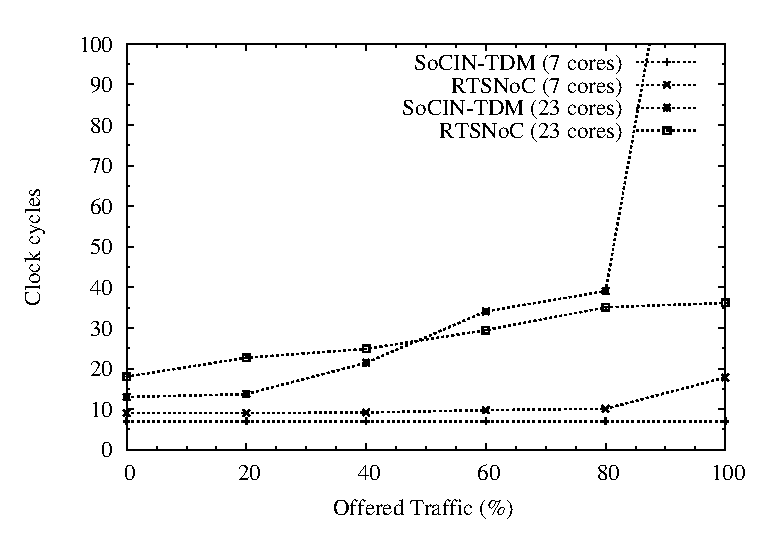
\includegraphics[width=.80\columnwidth]{Figures/latency}
}
\quad
\subfloat[Jitter variance \textit{vs.} offered traffic for SoCIN-TDM and RTSNoC networks.]{
	\label{jitter}
	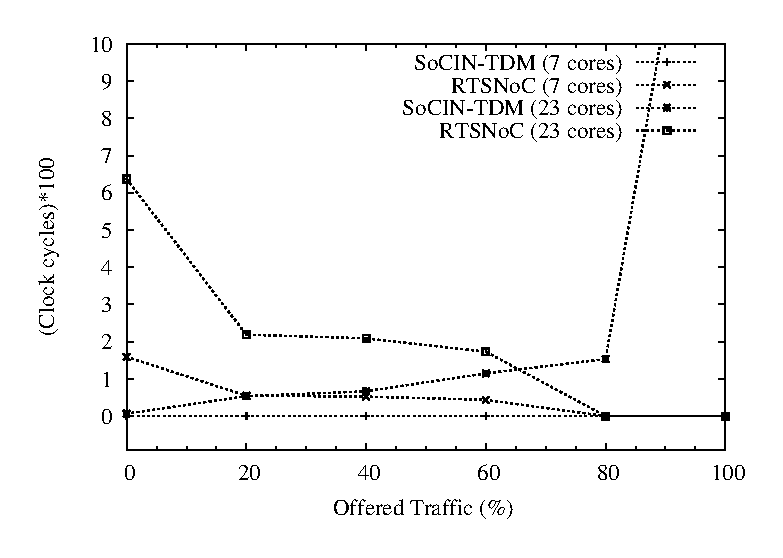
\includegraphics[width=.80\columnwidth]{Figures/jitter}
}

\caption{Latency and jitter results.}
\label{fig:latresults}
\end{figure*}

\subsection{Latency and jitter}

The performance of a NoC is usually given by its latency. However, another important criterion for
real-time applications is jitter. With small jitter it is possible to establish lower bounds on
the WCET of the system. To evaluate these metrics, four networks, composed by routers from
SoCIN-TDM network and RTSNoC network were built and split in two scenarios, as shown in Figure
\ref{Experiments_Platforms}. \emph{Traffic generators}~(TG) cores generate random amounts of
packets at random time periods. All packets are sent to a \emph{traffic measurement}~(TM) core which
measures the latency and jitter for each TG.

\figSC{.36}{Experiments_Platforms}
{Networks used for latency and jitter evaluation: (A) SoCIN-TDM with 7
cores; (B) RTSNoC with 7 cores, (C) SoCIN with 23 cores, and (D) RTSNoC with 23 cores.}

Thirty consecutive measurements of latency were done for different fractions of the total traffic capacity (20, 40, 60, 80 and 100\%). Figure \ref{latency} shows the results. The SoCIN-TDM network
keeps the latency constant for scenario I since it was designed to offer constant latency
(the number of hops is less than the number of TDM channels for that network size). 
When the network
is increased to receive new cores as shown in scenario II, the limited number of available TDM
channels causes contention, resulting in a significant increase in latency. The RTSNoC, on the other
hand, keeps the latency under control even at 100\% of network utilization. RTSNoC performs runtime scheduling of the flows that are competing for some communication channel, meaning that all flows may have access to all channels over time.

Figure \ref{jitter} shows the average jitter values. As expected for scenario I, the SoCIN-TDM
network has a constant jitter due to the availability of enough TDM channels. When the NoC connects
more cores in scenario II, the jitter grow significantly. On the other hand, the jitter for RTSNoC
is high under low traffic and tends to decrease as the traffic increases. In RTSNoC, with low
traffic the probability of a flow being randomly preempted increases, thus increasing the jitter.
In the extreme case of 100\% of traffic, however, all flows are competing for the same resources
full-time, keeping the scheduling policy constant. For over 80\% of traffic, RTSNoC has the
same null jitter presented by SoCIN-TDM in scenario~I.
%\figSC{.65}{jitter}
%{Jitter variance \textit{vs.} offered traffic for SoCIN-TDM and RTSNoC networks}
%\todo[inline]{Provide a summary of the area, latency and jitter results, and justify why RTSNoC would be better in each of the situations}
As shown in this Section,  RTSNoC is an effective solution to make real SoCs. The SoC implemented with RTSNoC has a lower silicon consumption, when compared to a TDM based NoC. Furthermore, RTSNoC does not need to consume more silicon resources to deal with an increase in the traffic flow, due its performance in high traffic in terms of latency and jitter.

\section{Case study}
\label{sec:case_study}

In order to evaluate the performance of RTSNoC in an industrial application with real-time
constraints, we have used it as the base infrastructure for deploying a \textit{Private Automatic Branch eXchange}~(PABX) SoC.
%The PABX SoC shown in Figure \ref{RTSNoC_Figure_15} targets FPGA-based telecommunication systems and
The PABX SoC targets FPGA-based telecommunication systems and consists of an RTSNoC router interconnecting telecommunications processors.
The minimum features to implement the digital PABX are as follows: a 425 $Hz$ generator; a DTMF generator; a digital switch that provides conference service for voice calls; a DTMF detector; a softcore processor that works as the system controller; an interface to E1 link; and finally an interface to provide access to the PABX subscribers.

\figSC{.45}{RTSNoC_Figure_15}
{Block diagram showing the internal structure of the PABX SoC implemented using RTSNoC. Squares are used to represent cores with external interfaces.}



The core \emph{System Timer} generates a packet every 125 $\mu s$ which is sent to all other cores
connected to the router. This packet is an indication of a synchronization pulse to the system and, due
to network traffic conditions, its arrival may present jitter. However, the jitter is
always between known and tolerable limits for the PABX system, since the adoption of the packet
structure ensures that no single flow will retain the communication channels indefinitely. 

%\subsection{Results}

The SoC was once again synthesized using the Xilinx's ISE version 13.1 targeting a Virtex 6 FPGA. 
The PABX system was analyzed in its maximum operation load. For this scenario, thirty two telephone
calls were generated at \emph{E1 link} and sent to \emph{Subscribers interface}. The incoming calls
were randomly generated and have short and random duration. For each incoming call, the PABX cores
exchange messages related to call identification, DTMF signaling generation and detection, and
call forward.

The RTSNoC had a clock frequency of a 100 $MHz$ with  maximum throughput of $133,312$ $Mbps$.
The processors generate data at approximately 16 $Mbps$.
Despite being a relatively low traffic in respect to the total network capacity, message exchanges occurs in bursts soon after the identification a
synchronization message from the clock System (\emph{System Timer} on WW port). Thus, there is intense
competition for resources during a short period, creating jitter for the synchronization packets.
Several measures were performed to evaluate the jitter in the synchronization packets. 

Figure \ref{RTSNoC_Figure_17} shows the latency variation of synchronization packets received at port
NW. All measured latency was between 317 $ns$ and 288 $ns$, with an average value of 302
$ns$, matching the 420 $ns$ WCET that can be obtained from Equation \ref{eq:total_latency}.

\figSC{.50}{RTSNoC_Figure_17}
{Latency of synchronization packets at port NW.}


\section{Conclusion}
\label{sec:conclusion}

We present a predictable real-time NoC called RTSNoC. 
RTSNoC enables simple and accurate worst-case latency analysis to determine the upper bound on communication latencies. 
The router design can connect up to eight cores or it can be connected to other routers to build a regular 2-D mesh network. 
We use a dynamic priority-based algorithm that keeps uniform and known network latency for any network load. 
This is possible since all flits include routing information, which allows the preemption of any data flow and avoids network contention. 
We show how to compute the worst-case latencies, and we implement RTSNoC on an FPGA.
Our experimental show that the latency is within the bounds determined by our analysis in all evaluated scenarios.
We also use the RTSNoC as the interconnect for a PABX SoC. 
The latency introduced by the NoC showed well-defined behavior, allowing the creation of local logic clocks in a relatively straightforward way.
Furthermore, RTSNoC showed significant differences in terms of silicon area when compared with
contention-based a TDM NoC. 
RTSNoC has a high relative area cost when used to connect a small number of cores; however, the relative area is significantly reduced when RTSNoC is used to build large
SoCs.
Through this, we confirm that RTSNoC is a low cost, and scalable solution for the interconnection of complex SoCs for real-time applications.

\iffalse
\section{Acknowledgments}
We would like to thank the authors of SoCIN network for providing the source code of their NoC, and
Intelbras S.A. for providing the PABX hardware platform used in our evaluation.
\fi


\bibliographystyle{IEEEtran}
\bibliography{rtsnoc}

\end{document}

